\documentclass[11pt,a4paper]{article}

% ---------------------------------------------------------------------------
% Energy service and peroxide handling in a proteome-constrained red-cell
% model: exact inventory certificates, a certified turnover plateau, and
% kinetic limits.
%
% Author metadata: set the macros below before submission.  Author and
% affiliation are deliberately blank in this version.
% ---------------------------------------------------------------------------
\newcommand{\PaperAuthor}{}
\newcommand{\PaperAffiliation}{}
\newcommand{\PaperDate}{16 September 2026}

\usepackage[T1]{fontenc}
\usepackage[utf8]{inputenc}
\usepackage{lmodern}
\usepackage{microtype}
\usepackage[a4paper,margin=1.05in]{geometry}
\usepackage{amsmath,amssymb,amsthm,mathtools}
\usepackage{booktabs}
\usepackage{array}
\usepackage{enumitem}
\usepackage{longtable}
\usepackage{graphicx}
\usepackage{xcolor}
\usepackage{capt-of}
\usepackage[obeyspaces,spaces]{url}
\usepackage[numbers,sort&compress]{natbib}
\usepackage[colorlinks=true,linkcolor=blue!55!black,citecolor=blue!55!black,urlcolor=blue!55!black]{hyperref}
\hypersetup{pdftitle={Energy service and peroxide handling in a proteome-constrained red-cell model},
  pdfkeywords={red blood cell, genome-scale metabolic model, proteome constraints,
    linear programming certificate, exact rational arithmetic, glutathione,
    catalase, hydrogen peroxide, carrier recycling, formal verification, Lean}}

\DeclareUrlCommand\lean{\urlstyle{tt}}
% A 64-character digest, given in four 16-character pieces so that it may break
% across lines.  The pieces are concatenated with no separator.
\newcommand{\hashfour}[4]{\texttt{#1\allowbreak#2\allowbreak#3\allowbreak#4}}
\setlist{itemsep=2pt,topsep=3pt}
\setlength{\emergencystretch}{1.5em}

\theoremstyle{plain}
\newtheorem{theorem}{Theorem}[section]
\newtheorem{proposition}[theorem]{Proposition}
\newtheorem{lemma}[theorem]{Lemma}
\newtheorem{corollary}[theorem]{Corollary}
\theoremstyle{definition}
\newtheorem{definition}[theorem]{Definition}
\theoremstyle{remark}
\newtheorem{remark}[theorem]{Remark}

\newcommand{\R}{\mathbb R}
\newcommand{\dd}{\mathrm d}
\newcommand{\Nc}{N_{\mathrm c}}
\newcommand{\Na}{N_{\mathrm a}}
\newcommand{\Ctot}{C_{\mathrm{tot}}}
\newcommand{\mmolg}{\mathrm{mmol}\,\mathrm{gDW}^{-1}}
\newcommand{\rx}[1]{\textnormal{\textsc{#1}}}

\title{Energy service and peroxide handling in a proteome-constrained
red-cell model:\\ exact inventory certificates, a certified turnover plateau,\\
and kinetic limits}
\author{\PaperAuthor\\[2pt] {\small\itshape \PaperAffiliation}}
\date{\PaperDate}

\begin{document}
\maketitle

\begin{abstract}
Whether stored red cells can sustain an ATP-dependent service while consuming
an oxidative challenge is usually approached through a metabolic flux envelope.
We ask what such an envelope actually decides. Working with the
proteome-constrained S7 instance of RBC-GEM under an explicit finite-horizon
relaxation, we prove three exact statements about one concrete model. First, a
complete source-matrix inventory certificate: for every cumulative extent
vector obeying the declared bounds, balances and terminal floors, the weighted
combination of Na/K-ATPase service $M$ and two-route peroxide turnover $Q$
obeys $M+4Q\le w^{\top}(x_0-\ell)+25.439042\,T+4(R_{\rx{cysglth}}+
R_{\rx{lhcystin}}+R_{\rx{ssgthrd}})$, with all $19\,620$ columns and their
decimal coefficients retained; the concrete vector inequality is verified in
Lean~4. Second, and in a deliberately restricted diagnostic medium, an exact
rational primal witness together with two exact dual certificates shows that
the optimal turnover is uniformly enclosed,
$6.50048030\le F(m)\le 6.50048050$ $\mmolg$, for \emph{every} required service
$0\le m\le 1.0345238$, while no feasible point at all has service above
$1.0345238944791832$. The certified interval therefore covers all but a window of width
$9\times10^{-8}$ of the attainable service range, and across it the variation of
the optimum is at most $1.93\times10^{-7}$, about $3\times10^{-6}$ percent of
the turnover level. Third, the apparent tradeoff reported when four internal reverse sulfur
directions are blocked is not reproduced by closing external sulfur supply: a
stoichiometric identity shows that the relevant carriers cancel against an
independent reductant, so supply accounting cannot bound repeated turnover.
We then show what the envelope does not decide. A returned optimum imports
$1000$ peroxide units and leaves $993.4995$ of them in the terminal pool;
minimising terminal peroxide merely diverts $981.05$ units through uncounted
haemoglobin reactions, and only a subsequent parsimony step removes the
gratuitous handling. Finite carrier pools supply the missing constraint, and we
prove a sharp finite-time recycling bound,
$V(T)\le\frac{ab}{a+b}\Ctot T+\frac{a}{a+b}(g(0)-\frac{b\Ctot}{a+b})
(1-e^{-(a+b)T})$, which is attained, implies the harmonic average-rate ceiling
with an $O(1/T)$ correction, and starts quadratically from a fully oxidised
pool. A complementary paired-signal recovery identity gives a necessary
consistency test for inferring integrated effective reduction from treated and
untreated assays. All results are conditional on the stated model instance;
a source-supported theorem of stored-cell oxidative tolerance with preserved
ATP-dependent function remains open, and we state precisely which measurements
would close it.
\end{abstract}

\section{Introduction}\label{sec:intro}

\subsection{The question}
A quantitative claim that a preparation of red cells tolerates an oxidative
challenge while preserving an ATP-dependent function needs five things: a
preparation, an initial inventory, a substrate supply, a rate law, and an
endpoint that separates useful peroxide handling from injury. A metabolic model
supplies some of these and not others. It can say which integrated combinations
of work and peroxide consumption obey its own resource and allocation
constraints. It does not by itself say whether finite carrier pools and
supported kinetics can realise such a combination on the required timescale,
nor whether the resulting trajectory preserves the function of interest.

Keeping those three questions apart is the organising principle of this paper.
We take one published proteome-constrained reconstruction of the human red
blood cell, add an explicit finite-horizon relaxation, and ask what follows
exactly. The answer is a set of conditional exclusion statements that are sharp
about the model and silent about the cell, together with an identification of
the specific assumptions that would have to be measured before the model could
speak about a challenge assay.

\begin{quote}
Which service--turnover restrictions follow exactly from one published
proteome-constrained red-cell model, and which additional assumptions are
needed before its flux envelope can be read as oxidative resilience?
\end{quote}

The source reconstruction is RBC-GEM with the enzyme information of its
supplementary file S6 and the proteome-constrained model of its supplementary
file S7 \citep{haiman2025}. The analysis below is an additional
finite-inventory use of those inputs. It is not a claim that the source
publication established stored-cell challenge tolerance, and no defect in that
work is alleged anywhere in this paper.

\subsection{Main results}
Section~\ref{sec:model} fixes the relaxation and the observables: $M$ is the
cumulative Na/K-ATPase turnover over a horizon $T$, and $Q=2\xi_{\rx{cat}}+
\xi_{\rx{gthp}}$ counts peroxide molecules consumed through catalase and the
glutathione-peroxidase column. Our results are the following.

\begin{enumerate}[label=(\roman*)]
\item \emph{A complete inventory certificate} (Theorem~\ref{thm:inventory}).
For the explicit S7 matrix, all $19\,620$ columns, the declared sink closure
and every source decimal read as a rational number,
\[
M+4Q\ \le\ w^{\top}(x_0-\ell)+25.439042\,T
+4\bigl(R_{\rx{cysglth}}+R_{\rx{lhcystin}}+R_{\rx{ssgthrd}}\bigr),
\]
where $w\ge0$ has $53$ nonzero chemical entries and $R_j$ is the negative part
of the net cumulative extent of reaction $j$. The exact time coefficient is a
rational number below $25.439042$, displayed in \eqref{eq:kappa}. The concrete
finite vector inequality compiles in Lean~4.

\item \emph{Recycling defeats supply accounting}
(Section~\ref{sec:recycling}). Blocking four internal reverse sulfur directions
produces a declining numerical service--turnover frontier of slope $-1/4$; that
effect is \emph{not} reproduced by closing all $56$ identified sulfur-containing
exchange imports. The reason is an exact stoichiometric identity: the chemical
parts of $\rx{hcystrdx}+\rx{trdry}-\rx{lhcystin}+\rx{gthp}-\rx{estronedhy}$
sum to $\text{estradiol}+\mathrm H_2\mathrm O_2\to\text{estrone}+
2\,\mathrm H_2\mathrm O$, with every sulfur, thioredoxin and nicotinamide
carrier cancelling. A budget on carrier \emph{uptake} cannot bound carrier
\emph{reuse}.

\item \emph{A plateau certified over the whole service range}
(Theorem~\ref{thm:plateau}). In a restricted diagnostic medium, one exact
rational feasible point and two exact dual certificates give
\[
6.50048030\ \le\ F(m)\ \le\ 6.50048050\ \mmolg
\qquad\text{for every }0\le m\le 1.0345238 ,
\]
where $F(m)$ is the maximal turnover subject to service at least $m$, together
with the exact ceiling $M\le 1.0345238944791832$ for every feasible point. The
certified endpoint is $99.99999\%$ of that ceiling, so the statement covers all
but a window of width $9\times10^{-8}$ of the attainable range of $m$, rather
than a sampled sub-interval, and the variation of $F$ across the certified
interval is at most $1.93\times10^{-7}$. The general principle
behind this is a one-witness lemma (Lemma~\ref{lem:enclosure}): an enclosure
valid on an entire interval follows from a single feasible point plus a single
global upper certificate, with no grid. That lemma, the shape of the value
function and the ceiling argument are verified in Lean~4.

\item \emph{Turnover does not constrain peroxide burden}
(Section~\ref{sec:burden}). The returned optimum imports $1000$ units of
peroxide, counts $6.50048$ through the two routes and leaves $993.49952$ in the
terminal pool. Minimising terminal peroxide at fixed service and turnover
substitutes $981.05$ units of uncounted haemoglobin-peroxide consumption for
that accumulation; only a further parsimony step removes the gratuitous
handling and brings import down to the counted consumption. A terminal value is
not a burden ceiling, and none of these solutions carries a damage endpoint.

\item \emph{A sharp finite-time carrier bound} (Theorem~\ref{thm:carrier}).
For a closed two-state carrier with total amount $\Ctot$, reduced amount $g$,
oxidation $v\le ag$ and regeneration $u\le b(\Ctot-g)$,
\[
V(T)=\int_0^T v\ \le\ \frac{ab}{a+b}\,\Ctot T
+\frac{a}{a+b}\Bigl(g(0)-\frac{b\,\Ctot}{a+b}\Bigr)\bigl(1-e^{-(a+b)T}\bigr),
\]
and the bound is attained. It requires no terminal condition, it implies the
harmonic average-rate ceiling $V(T)/T\le \Ctot/(1/a+1/b)$ with an $O(1/T)$
correction, and for an initially fully oxidised pool it starts as
$\tfrac12ab\,\Ctot T^2$: regeneration must precede oxidation. This is the
smallest additional structure that separates the stoichiometric feasibility of
repeated recycling from its kinetic feasibility, and the S7 instance shows that
the separation matters, since the certified witness recycles carriers whose
modelled initial amount is zero. The inequality is verified in Lean~4.

\item \emph{A recovery consistency test} (Section~\ref{sec:recovery}). For
paired treated and untreated signals with a common initial value and a constant
residual-input fraction $r$, the transformed signal
$z=(C_s-rD)/((1-r)D_0)$ equals $e^{-\int_0^tk}$ exactly, for arbitrary
time-varying oxidative input. Hence $z$ is positive, bounded by one and
nonincreasing, which is a falsifiable requirement on paired observations, and
an explicit discrepancy bound converts an observation interval into an interval
for the integrated effective reduction.
\end{enumerate}

\subsection{What this paper does not establish}
Every statement above is conditional on a declared model instance. None of them
establishes an admissible human preparation, a tolerable external dose, a
kinetic trajectory, or a clinical threshold. In particular the coefficient $4$
in (i) is a certificate weight, not a universal ATP cost of removing a peroxide
molecule; the potential $w^{\top}x$ is a mathematical resource account, not a
Gibbs energy; and the flatness in (iii) is a property of one restricted
diagnostic medium, not a demonstration that storage energy and oxidative
resilience are unrelated in real cells. The original biological target, a
source-supported theorem of stored-cell oxidative tolerance with preserved
ATP-dependent function, remains open; Section~\ref{sec:discussion} states the
smallest extension we think could close it.

\subsection{Evidence classes}
Different results in this paper rest on different kinds of evidence, and we
label them explicitly rather than letting the strongest label spread.

\begin{center}
\small
\begin{tabular}{@{}p{0.30\textwidth}p{0.27\textwidth}p{0.36\textwidth}@{}}
\toprule
Result & Evidence class & Boundary \\
\midrule
Inventory certificate, Theorem~\ref{thm:inventory} &
Lean~4 kernel check of the concrete vector inequality, plus an exact
source-data audit &
XML parsing, reaction-name interpretation and biological admissibility are
external premises \\
Uniform enclosure, Lemma~\ref{lem:enclosure} and
Propositions~\ref{prop:shape}--\ref{prop:ceiling} &
Ordinary proofs, also verified in Lean~4 &
Nothing model-specific \\
Plateau instance, Theorem~\ref{thm:plateau} &
Exact rational primal and dual audit in Python &
Not claimed as a Lean-replayed source certificate \\
Carrier bounds, Theorem~\ref{thm:carrier} and corollaries &
Ordinary analytic proofs, verified symbolically; the main inequality is also
verified in Lean~4 for everywhere-differentiable $g$ &
Coefficients $a,b,\Ctot$ are not calibrated for any preparation \\
Recovery identity and error bounds, Section~\ref{sec:recovery} &
Lean~4 for the identity, the discrepancy bound and the logarithmic interval &
No validated intervention model; no reanalysis of donor data \\
Numerical optima, sensitivities and cleanup &
Floating-point linear programs &
Feasibility of a relaxation, not kinetic realisability \\
\bottomrule
\end{tabular}
\end{center}

\subsection{Relation to existing work}
None of the ingredients is individually new, and we claim no new duality
theory. Flux balance analysis and its envelope calculations are standard
\citep{orth2010}. Non-steady intracellular accounting has direct prior art in
unsteady-state FBA, which uses quantitative time-course metabolomics to
constrain changing pools and relaxes unmeasured nodes when required
\citep{bordbar2017}; our finite-inventory relaxation uses much less dynamic
information and consequently establishes much less about trajectories. Dynamic
FBA couples metabolic optimisation to changing extracellular conditions
\citep{mahadevan2002}, and personalised kinetic red-cell models address a
different, more dynamically specified inference problem
\citep{bordbar2015}. Selecting among optimal flux distributions by a parsimony
criterion is established practice \citep{lewis2010}, and thermodynamic or
loopless constraints remove certain unsupported internal cycles
\citep{schellenberger2011}; neither addresses finite carrier abundance or a
substrate-powered recycling route, which is the obstruction we isolate in
Section~\ref{sec:recycling}. The paired-signal cancellation in
Section~\ref{sec:recovery} is an integrating-factor argument of a familiar
kind.

What is specific here is the concrete instance and its traceability: a complete
exact audit of a named published model, at stated premises, with the decisive
inequality verified by a proof kernel; an enclosure that holds uniformly over
an entire certified service interval rather than at sampled points; and a
diagnosis of which modelling assumptions actually move the answer.

\section{The model instance}\label{sec:model}

\subsection{Finite-horizon relaxation}
Partition the expanded source matrix into chemical rows $\Nc$ and auxiliary
allocation rows $\Na$. Let $\xi\in\R^{19620}$ be the vector of net signed
cumulative reaction extents over a horizon $T\ge0$, let $x_0$ be the initial
chemical amounts, $\ell$ the required terminal chemical floors, and $L_j,U_j$
the source lower and upper rate bounds. The relaxation is
\begin{equation}\label{eq:relax}
x_0+\Nc\xi\ \ge\ \ell,\qquad \Na\xi=0,\qquad
L_jT\le\xi_j\le U_jT,\qquad T\ge 0 .
\end{equation}
The expanded S7 instance has $19\,620$ columns and $10\,411$ rows, of which
$2\,157$ are chemical and $8\,254$ are auxiliary. Auxiliary rows encode enzyme
allocation and proteome budgets; they are algebraic relations, not inventories
of ordinary chemicals, and must never be described as terminal amounts of
metabolites. Following the model experiments of the source-model audit, imports
through every sink reaction except the three ionic sinks for sodium, potassium
and calcium are closed, while exports remain allowed and the exchange feed
bounds retain their source values integrated over $T$.

Two features of \eqref{eq:relax} deserve emphasis because the conclusions
depend on them. Terminal floors are necessary conditions only: they constrain
neither intermediate availability nor any rate law. And signed extents are
equivalent to splitting reversible directions, so using them discards no sign
or bound information.

The principal diagnostic family takes $T=1$~hour, zero terminal floors and zero
initial chemical stocks. This is an algebraic diagnostic family and not a
viable initial red-cell state; in particular it can admit balanced turnover
without the carrier inventory needed to start it, which is exactly the gap
quantified in Section~\ref{sec:carrier}.

\subsection{Observables}
Write
\begin{equation}\label{eq:obs}
M=\xi_{\rx{nakt}},\qquad Q=2\xi_{\rx{cat}}+\xi_{\rx{gthp}},\qquad
R_j=\max\{-\xi_j,0\}.
\end{equation}
The Na/K-ATPase column consumes one ATP per turnover; catalase consumes two
peroxide molecules per extent and the glutathione-peroxidase column consumes
one, and both source directions are nonnegative. Thus $Q$ is a peroxide
equivalent through two specified routes. It is not total peroxide
disappearance, not total antioxidant capacity, and not a damage-free challenge
dose. The reverse quantity $R_j$ is the negative part of the \emph{net}
cumulative extent; if a reaction changes direction inside the interval its
gross reverse turnover may exceed $R_j$, so any justified bound on gross
reverse turnover also bounds $R_j$, if less sharply.

\subsection{Units}
\begin{center}
\small
\begin{tabular}{@{}ll@{}}
\toprule
Quantity & Unit or convention \\
\midrule
Chemical rate; horizon & $\mathrm{mmol}\,\mathrm{gDW}^{-1}\mathrm h^{-1}$; hours \\
Chemical amount, net cumulative extent & $\mmolg$ \\
$M$, $Q$ in the one-hour experiments & cumulative amounts in $\mmolg$ \\
Source protein abundance & $\mathrm{nmol}\,\mathrm{gDW}^{-1}$; auxiliary columns keep their encoded scales \\
Carrier coefficients $a,b$ & $\mathrm h^{-1}$ \\
Concentration & amount divided by a measured solution volume per gDW \\
\bottomrule
\end{tabular}
\end{center}

Because $T=1$~h in the numerical experiments, $M$ and $Q$ are numerically equal
to the corresponding average rates; they remain amounts. No compatible water
volume is supplied for the peroxide diagnostics below, so a reported terminal
peroxide value of $993.5$ is $993.5\ \mmolg$ and \emph{not} $993.5$~mM. Turning
it into a concentration requires a justified compartment volume together with
explicit conversions among packed-cell volume, cell water, haemoglobin mass and
dry mass.

\subsection{Two declared media}\label{sec:media}
Results below use two constraint sets. The \emph{original feed envelope} is
\eqref{eq:relax} with the sink closure just described. The \emph{restricted
diagnostic medium} additionally closes the $56$ identified sulfur-containing
exchange imports and the $435$ carbon-containing exchange imports, with the
named D-glucose, carbon-dioxide and bicarbonate exchanges retained. Membership
is decided by the source chemical formulas together with the actual singleton
exchange stoichiometry; the two closure sets overlap, so $56$ and $435$ must
not be added. Exact reaction identifiers matter: only the named D-glucose
exchange \lean{R_EX_glc__D_e} is retained, and the source's separately encoded
glucose anomer exchanges must not be silently merged. Other permitted inorganic
exchanges remain open and some formulas are unknown, which limits what the
phrase ``restricted medium'' can mean. It is a declared diagnostic, not a
reconstruction of any experimental buffer.

\section{A complete finite-inventory certificate}\label{sec:certificate}

\begin{theorem}[Source-model inventory bound]\label{thm:inventory}
Let $\xi$ satisfy \eqref{eq:relax} for the explicit S7 matrix and the original
feed envelope of Section~\ref{sec:media}, with $T\ge0$. Then, with the
certificate vectors of Appendix~\ref{app:repro},
\begin{equation}\label{eq:main}
M+4Q\ \le\ w^{\top}(x_0-\ell)+25.439042\,T
+4\bigl(R_{\rx{cysglth}}+R_{\rx{lhcystin}}+R_{\rx{ssgthrd}}\bigr),
\end{equation}
where $w\ge0$ has $53$ nonzero chemical entries, among them $2$ for ATP, $1$
for ADP, $2$ for reduced glutathione and $1$ for haemoglobin-bound
2,3-DPG.
\end{theorem}

\begin{proof}
Let $c^{\top}\xi=M+4Q$, so that the only nonzero objective coefficients are
$c_{\rx{nakt}}=1$, $c_{\rx{cat}}=8$ and $c_{\rx{gthp}}=4$. The certificate
supplies nonnegative chemical weights $w$, signed auxiliary weights $y$ with
$290$ nonzero entries, and nonnegative supply coefficients $\alpha$ equal to
$4$ on the three displayed sulfur columns and zero elsewhere. For each column
put
\begin{equation}\label{eq:residual}
d_j=c_j+\alpha_j+w^{\top}N_{\mathrm c,j}-y^{\top}N_{\mathrm a,j},
\qquad
\kappa=\sum_j\max\{d_jL_j,\ d_jU_j\}.
\end{equation}
Three elementary facts finish the argument. For a signed extent inside its
interval and $T\ge0$ we have $d_j\xi_j\le T\max\{d_jL_j,d_jU_j\}$, by cases on
the sign of $d_j$. For a nonnegative supply coefficient,
$-\alpha_j\xi_j\le\alpha_j\max\{-\xi_j,0\}=\alpha_jR_j$. And summing the exact
column identities gives
\[
c^{\top}\xi=-w^{\top}\Nc\xi+y^{\top}\Na\xi+\sum_j(d_j-\alpha_j)\xi_j
\ \le\ w^{\top}(x_0-\ell)+\kappa T+\sum_j\alpha_jR_j ,
\]
where nonnegativity of $w$ together with the chemical floors of
\eqref{eq:relax} bounds the first term, and the auxiliary balances annihilate
the second. Evaluating \eqref{eq:residual} over all $19\,620$ source columns
with every decimal read as an exact rational number gives
\begin{equation}\label{eq:kappa}
\kappa=\frac{1283461673726143619667945455169487587}
{50452437500000000000000000000000000}
=25.439041943734505\ldots\ <\ 25.439042 ,
\end{equation}
and rounding the coefficient upward proves \eqref{eq:main}.
\end{proof}

Two aspects of this proof are worth isolating. No optimisation algorithm is
assumed correct anywhere: verifying a supplied upper certificate needs neither
strong duality nor optimality of any solver output, only the three inequalities
above. And the three priced sulfur columns keep their residual $-4$, so their
reverse directions remain permitted and appear explicitly in the bound rather
than being forbidden. A fourth reaction restricted in an early diagnostic,
\lean{HTSULGTHST}, has residual zero in this certificate; restoring its
direction while retaining the other three restrictions left both tested
endpoint optima unchanged, exactly as the coefficient analysis predicts.

\begin{corollary}\label{cor:exclusion}
Suppose independently justified budgets give $w^{\top}(x_0-\ell)\le I$ and
$R_{\rx{cysglth}}+R_{\rx{lhcystin}}+R_{\rx{ssgthrd}}\le S$. Then a service
requirement $M\ge m$ forces
\begin{equation}\label{eq:tradeoff}
Q\ \le\ \frac{I+25.439042\,T+4S-m}{4} .
\end{equation}
If the right-hand side is negative, the service requirement and the
nonnegative-turnover assumption are jointly infeasible under those premises.
\end{corollary}

The corollary is a useful exclusion only when $I$ and $S$ have independent
support. That the right-hand side decreases in $m$ does not by itself exhibit a
biological tradeoff: the inequality may be loose, and the internal reverse
budget may itself depend on the protocol. Nor does exact arithmetic upgrade
estimated enzyme capacities, an assumed medium or uncertain initial inventories
into exact biological facts; it controls only the arithmetic of the stated
model. Finally, being below the bound constructs nothing. Theorem~\ref{thm:inventory}
excludes; it does not produce a trajectory, control a peroxide burden, or show
that ATP is preserved throughout the interval.

\section{Recycling defeats supply accounting}\label{sec:recycling}

The first discriminating experiment asked whether finite inventory alone
exposes a service--turnover tradeoff in the original envelope. It does not.
Over the sampled original-direction family the optimal $Q$ is constant at
$46.93124973$ while the required service ranges over $[0,3.6422153]$. Blocking
four internal reverse sulfur directions (\lean{CYSGLTH}, \lean{LHCYSTIN},
\lean{HTSULGTHST}, \lean{SSGTHRD}) produces instead a frontier of slope
approximately $-1/4$, descending from $6.3597605$ to $5.4492067$ across the
same service range. That restriction was a diagnostic intervention in the
model. It is not an experimental finding that those directions vanish in stored
cells, and the induced tradeoff should not be reported as a property of the
reconstruction.

The natural repair is to price sulfur where it enters the cell rather than
where it turns over internally. It fails, for a reason worth recording.
Closing all $56$ sulfur-containing exchange imports lowers the optimum only
from $46.93125$ to $35.07139$, and leaves it unchanged as the service
requirement rises (Table~\ref{tab:media}). A structured replacement certificate
that assigns weights to cysteine, homocysteine and hydrosulfide pools does
cancel the three targeted residuals exactly, but it changes $34$ columns and
degrades the rate coefficient from $25.44$ to approximately $10\,492.57$, of
which $4000$ comes from the extracellular $\mathrm H_2\mathrm S$ dissociation
column alone, because the candidate weights hydrosulfide and not
$\mathrm H_2\mathrm S$. Chemically interconverting protonation states must be
weighted consistently unless their imbalance is deliberately budgeted.

\begin{table}[t]
\centering
\small
\begin{tabular}{@{}lrl@{}}
\toprule
Declared constraints & Required service $m$ & Optimised $Q$ \\
\midrule
Original feed envelope & $0$ to $3.64222$ & $46.93125$ at all tested points \\
Sulfur exchange imports closed & $0$ and $3.64222$ & $35.07139$ at both endpoints \\
Four internal reverse directions blocked & $0$; $3.64222$ & $6.35976$; $5.44921$ \\
Restricted carbon and sulfur feeds & $0$; $1.02418$ & $6.50048$; $6.50048$ \\
Same restricted feeds, old demand & $3.64222$ & infeasible without any challenge \\
\bottomrule
\end{tabular}
\caption{Numerical optima at a one-hour horizon under four declared constraint
sets, in $\mmolg$. These are floating-point optima of the stated relaxation.
The internal-direction restriction is a model intervention and is distinct from
the external-supply restrictions. Each medium has its own service scale: the
restricted medium's service ceiling is $1.0345239$, so the old demand
$3.64222$ is infeasible there for reasons that have nothing to do with a
peroxide requirement.}
\label{tab:media}
\end{table}

The deeper obstruction is structural. In a sulfur-closed witness, glutathione
regeneration runs through reverse \lean{LHCYSTIN} coupled to \lean{HCYSTRDX}
and \lean{TRDRy}, and reverse \lean{ESTRONEDHy} supplies $23.40156$ of the
$28.17063$ NADPH units that \lean{TRDRy} consumes. Summing the chemical parts
of
\begin{equation}\label{eq:identity}
\begin{aligned}
&\rx{hcystrdx}+\rx{trdry}-\rx{lhcystin}+\rx{gthp}-\rx{estronedhy} \\
&\qquad\text{gives}\qquad
\text{estradiol}+\mathrm H_2\mathrm O_2\longrightarrow
\text{estrone}+2\,\mathrm H_2\mathrm O .
\end{aligned}
\end{equation}
Homocysteine, glutathione, thioredoxin and nicotinamide all cancel; eight
auxiliary enzyme terms do not cancel and are retained separately. This is a
chemical stoichiometric identity, not a self-contained feasible cycle of the
expanded model and not an observed human pathway. Its content is that a carrier
can be reused indefinitely while the net conversion is paid for by a different
reductant, so a budget on sulfur \emph{uptake} cannot bound sulfur-carrier
\emph{turnover}. Consistently with this reading, removing steroid imports does
not restore a tradeoff: the witness simply switches supply routes, with
\lean{G6PDH2} and \lean{GND} each contributing $0.53024$ to support
\lean{TRDRy} at $1.06047$ while \lean{GTHOx} contributes $2.19940$.

Two cautions. This is not automatically a thermodynamically impossible internal
loop, since a carrier cycle with a net external substrate conversion is not an
unpowered closed flux loop, and removing cycles indiscriminately would delete
legitimate catalysis along with possible artefacts \citep{schellenberger2011}.
And the failure of this particular replacement certificate does not show that
no better potential exists; it shows that the missing constraint is about
carrier abundance and rates, which is what Section~\ref{sec:carrier} supplies.

\section{A plateau certified over the whole service range}\label{sec:plateau}

\subsection{One witness and one certificate suffice}
Equal floating-point optima at two service levels suggest a plateau but prove
nothing between them. The following elementary lemma removes the temptation to
certify a grid: an enclosure valid on an entire interval follows from one
feasible point and one global upper bound.

Let $P\subseteq\R^n$ be a feasible set and $M,Q:\R^n\to\R$ two observables.
For $m\in\R$ write $P_m=\{\xi\in P: M(\xi)\ge m\}$ and let
\begin{equation}\label{eq:F}
F(m)=\max\{Q(\xi):\xi\in P_m\}
\end{equation}
whenever the maximum exists.

\begin{lemma}[Uniform enclosure from one witness]\label{lem:enclosure}
Suppose $Q(\xi)\le U$ for every $\xi\in P$ with $M(\xi)\ge0$, and suppose there
is $\xi_h\in P$ with $M(\xi_h)\ge m_h\ge 0$ and $Q(\xi_h)\ge L$. Then for every
$0\le m\le m_h$ the set $P_m$ is nonempty and
\[
L\ \le\ F(m)\ \le\ U .
\]
\end{lemma}

\begin{proof}
Fix $0\le m\le m_h$. Since $M(\xi_h)\ge m_h\ge m$, the witness lies in $P_m$,
so $P_m\ne\emptyset$ and $F(m)\ge Q(\xi_h)\ge L$. If $F(m)$ is attained at
$\xi\in P_m$ then $M(\xi)\ge m\ge0$, so the upper certificate applies and
$F(m)=Q(\xi)\le U$.
\end{proof}

Lemma~\ref{lem:enclosure} is verified in Lean~4 as
\lean{PlateauEnclosure.uniform_enclosure}, with the feasibility half separated
as \lean{feasible_nonempty}. It is deliberately stated for any attained
maximum, so no compactness hypothesis is hidden in the notation; in the application $P$ is a nonempty
compact polytope, so the maxima exist. Two further elementary facts describe
the shape of $F$ and the domain on which the question is meaningful.

\begin{proposition}\label{prop:shape}
$F$ is nonincreasing on its domain. If moreover $P$ is convex and $M,Q$ are
linear, then $F$ is concave: for $m=am_1+bm_2$ with $a,b\ge0$ and $a+b=1$,
\[
F(m)\ \ge\ aF(m_1)+bF(m_2).
\]
\end{proposition}

\begin{proof}
If $m_1\le m_2$ then $P_{m_2}\subseteq P_{m_1}$, so $F(m_2)\le F(m_1)$. For
concavity let $\xi_i$ attain $F(m_i)$. Then $a\xi_1+b\xi_2\in P$ by convexity,
its service is $aM(\xi_1)+bM(\xi_2)\ge am_1+bm_2=m$, and its turnover is
$aF(m_1)+bF(m_2)$; hence it is a feasible competitor at level $m$.
\end{proof}

\begin{proposition}\label{prop:ceiling}
If $M(\xi)\le U_M$ for every $\xi\in P$, then $P_m=\emptyset$ for every
$m>U_M$.
\end{proposition}

Proposition~\ref{prop:shape} is verified in Lean~4 as
\lean{PlateauEnclosure.value_antitone} and \lean{value_concave}, and
Proposition~\ref{prop:ceiling} as \lean{infeasible_above_ceiling}.

Proposition~\ref{prop:ceiling} is what converts an enclosure on $[0,m_h]$ into
a statement about the \emph{whole} question: outside $[0,U_M]$ there is nothing
to enclose. The gap between the certified endpoint $m_h$ and the certified
ceiling $U_M$ is then the only part of the service axis left undecided, and in
the instance below it has width below $10^{-7}$.

\subsection{The S7 instance}
\begin{theorem}[Certified plateau and ceiling]\label{thm:plateau}
Let $P$ be the restricted-medium polytope of Section~\ref{sec:media} with
$T=1$~h, zero initial chemical stocks and zero terminal floors, retaining all
source bounds, directions and auxiliary balances. Then
\begin{equation}\label{eq:plateau}
6.50048030\ \le\ F(m)\ \le\ 6.50048050\ \mmolg
\qquad\text{for every } 0\le m\le 1.0345238 ,
\end{equation}
and $M(\xi)\le 1.0345238944791832$ for every $\xi\in P$, so $P_m=\emptyset$ for
$m>1.0345238944791832$.
\end{theorem}

\begin{proof}
Three exact objects are supplied and checked, and Lemma~\ref{lem:enclosure}
with Proposition~\ref{prop:ceiling} assembles them.

\emph{A rational witness.} An explicit rational vector $\xi_h$ with $1580$
nonzero entries is verified, in exact arithmetic and column by column, against
every source lower and upper bound, every chemical terminal floor and every
auxiliary equality. Its observables are
\[
M(\xi_h)=\frac{4421041890341877}{4273504273504270}=1.03452380234\ldots,
\]
\[
Q(\xi_h)=\frac{9400187505686245981195327946603}
{1446075838260537275756274164820}=6.500480304680\ldots,
\]
so $M(\xi_h)\ge 1.0345238$ and $Q(\xi_h)\ge 6.50048030$.

\emph{A turnover certificate.} Nonnegative chemical weights with $194$ nonzero
entries and signed auxiliary weights with $128$ nonzero entries give, by the
argument of Theorem~\ref{thm:inventory} with $c=Q$, $\alpha=0$, $x_0=\ell=0$,
\[
Q(\xi)\ \le\ U=\frac{81256006217701144379925098514861}
{12500000000000000000000000000000}=6.500480497416092\ldots
\]
for every $\xi\in P$, hence in particular whenever $M(\xi)\ge0$. Exactly eight
interval-cost terms are nonzero: four dominant enzyme-allocation terms
associated with \lean{GTHOx}, \lean{GND}, \lean{CAT} and \lean{G6PDH2}, and
four small residual terms at the corresponding metabolic columns. The small
terms are retained; describing the sum as containing only the four dominant
terms would be incorrect.

\emph{A service certificate.} The same construction with $c=M$ and a second
pair of weight vectors, with $200$ nonzero chemical and $251$ nonzero auxiliary
entries, gives
\[
M(\xi)\ \le\ U_M=\frac{2586309736197958070773983682319}
{2500000000000000000000000000000}=1.0345238944791832
\]
for every $\xi\in P$, with exactly two nonzero interval-cost terms, at
\lean{R_PYK} and at the pyruvate-kinase enzyme-allocation column
\lean{R_ENZDL_enzyme_PYK_total_pc}.

Lemma~\ref{lem:enclosure} with $m_h=1.0345238$, $L=6.50048030$ and $U$ as above
gives \eqref{eq:plateau} after rounding $L$ down and $U$ up;
Proposition~\ref{prop:ceiling} gives the emptiness claim.
\end{proof}

\begin{corollary}\label{cor:variation}
For $0\le m_1\le m_2\le 1.0345238$,
\[
0\ \le\ F(m_1)-F(m_2)\ \le\ U-L\ <\ 1.93\times10^{-7}\ \mmolg ,
\]
which is at most $3.0\times10^{-8}$ relative to the turnover level, that is
about $3\times10^{-6}$ percent.
\end{corollary}

\begin{remark}
The certified endpoint is $1.0345238$ and the certified ceiling is
$1.0345238944791832$, so \eqref{eq:plateau} covers a fraction
$0.99999990\ldots$ of the exactly certified service range. The residual window
of width $9.2\times10^{-8}$ is not certified; nothing in this paper asserts
what $F$ does there beyond the global upper bound $U$, which holds everywhere.
\end{remark}

\begin{remark}
Corollary~\ref{cor:variation} is an exclusion of a substantial objective
tradeoff \emph{within this model}, not an assertion of exact constancy and not
a statement of biological measurement precision. It also does not licence the
converse constructions: a requirement $Q>U$ is excluded in $P$, and a
requirement $Q\ge q$ with $q\le L$ together with $m\le 1.0345238$ is met by the
same witness, but neither statement establishes a tolerable external dose or
constructs a trajectory realising a prescribed exact value of $Q$.
\end{remark}

\subsection{How the certificate is found, and what decides it}
The generator starts from floating-point solver information to identify a
useful face and a candidate dual. Sparse rational elimination reconstructs the
active equalities, a small numerical program in the remaining nullspace locates
an interior candidate, and rational free parameters then determine a complete
rational vector. The final all-column rational audit decides feasibility; the
success or failure of the discovery program decides nothing. This separation
matters in practice as well as in principle: a first attempt that pushed the
witness to the extreme corner of the face, requesting $Q\ge6.50048049$, failed
the exact audit by about $4\times10^{-15}$ on $287$ columns, and the certified
statement is the one that survived the audit, not the one the solver reported.

Verifying a saved sparse primal and dual certificate costs one traversal of the
relevant matrix entries and bounds, so its arithmetic-operation count is
proportional to the sparse matrix size, with rational bit costs depending on
numerator and denominator sizes. The proof avoids certifying a dense service
grid. It establishes no new complexity result for finding certificates or for
solving linear programs in general.

\section{Turnover does not constrain peroxide burden}\label{sec:burden}

The returned restricted-medium optimum has $Q\approx6.5004805$, peroxide influx
$1000$ and terminal intracellular peroxide $993.4995195$, all as
source-normalised cumulative amounts. This follows directly from the peroxide
row: almost all imported peroxide simply remains, which the constraint set
permits because a terminal lower bound carries no protective upper bound.

A sequential cleanup shows that the accumulation is removable degeneracy rather
than a necessary feature of the optimum. Holding service and counted turnover
within $10^{-8}$ of their selected values and minimising terminal peroxide
drives the terminal pool to zero, but redirects approximately $981.05$ units
through two uncounted haemoglobin reactions, \lean{HBFE4ORPX} and
\lean{METHBPX}, at $490.52428$ each. Minimising total absolute flux while
retaining that result removes the gratuitous routes and brings the import down
to $6.50048$, matching the counted consumption exactly
(Table~\ref{tab:peroxide} and Figure~\ref{fig:two}A).

\begin{table}[t]
\centering
\footnotesize
\setlength{\tabcolsep}{4.5pt}
\begin{tabular}{@{}lrrrrp{0.21\textwidth}@{}}
\toprule
Saved stage & $M$ & $Q$ & influx & terminal & main uncounted consumption \\
\midrule
returned optimum & $0$ & $6.5004805$ & $1000$ & $993.4995195$ &
none in the peroxide trace \\
minimise terminal peroxide & $1.0241786$ & $6.5004805$ & $987.5490388$ & $0$ &
$490.5242791$ each through \lean{HBFE4ORPX} and \lean{METHBPX} \\
then minimise absolute flux & $1.0241786$ & $6.5004805$ & $6.5004805$ & $0$ &
the listed gratuitous routes disappear \\
\bottomrule
\end{tabular}
\caption{Peroxide accounting across three saved solutions, in $\mmolg$. The
rows are different primal vectors at different service values, obtained by
sequential objectives with a $10^{-8}$ tolerance; they are not one vector
viewed three ways. Service and turnover values are as recorded in the saved
result file.}
\label{tab:peroxide}
\end{table}

Three readings of this should be resisted. The solver did not hallucinate a
reaction or violate a supplied constraint: it optimised the problem it was
given, and the concern is that the problem leaves crucial outcomes
unconstrained. Haemoglobin-peroxide reactions are not intrinsically
meaningless; their large use in this particular optimum is gratuitous with
respect to the chosen objectives and may be consequential for damage, which is
a different and more interesting statement. And absolute-flux minimisation is a
selection rule whose result depends on the norm, the weights, reaction
splitting and the scaling of the expanded model, especially when chemical and
auxiliary columns are mixed; parsimonious flux selection has substantial prior
art \citep{lewis2010} and no claim of a uniquely justified physiological
objective is made here.

What a challenge-tolerance claim needs instead is an explicit endpoint. For a
compatible dynamic model with intracellular peroxide amount $H(t)$, a complete
balance has the form
\begin{equation}\label{eq:burden}
H(t)=H(0)+I_H(t)+P_H(t)-Q_{\text{counted}}(t)-Q_{\text{other}}(t)-E_H(t),
\end{equation}
with import $I_H$, internal production $P_H$, export $E_H$ and all remaining
consuming fates $Q_{\text{other}}$, every term on a consistent amount basis and
with the correct stoichiometric multiplicity. Some consuming fates represent
damage or irreversible loss of protective capacity. A zero value of $H(T)$
bounds neither $\sup_{t\le T}H(t)$, nor cumulative exposure, nor irreversible
injury. A tolerance claim therefore needs a supported burden ceiling, a damage
integral or a measured retained function, and the present model experiments
supply a numerical threshold for none of these.

Transport data alone do not close this gap either. Human red-cell peroxide
permeability has been measured at $37^{\circ}$C \citep{orrico2022}, but the
reported experiments include fresh cells and millimolar exposure, whereas the
stored-cell recovery assay considered in Section~\ref{sec:recovery} uses
micromolar peroxide. Temperature agreement is not transferability: membrane
area, dry-mass normalisation, concentration range and preparation must also
match before a permeability coefficient can be used to constrain an amount
flux.

\begin{figure}[t]
\centering
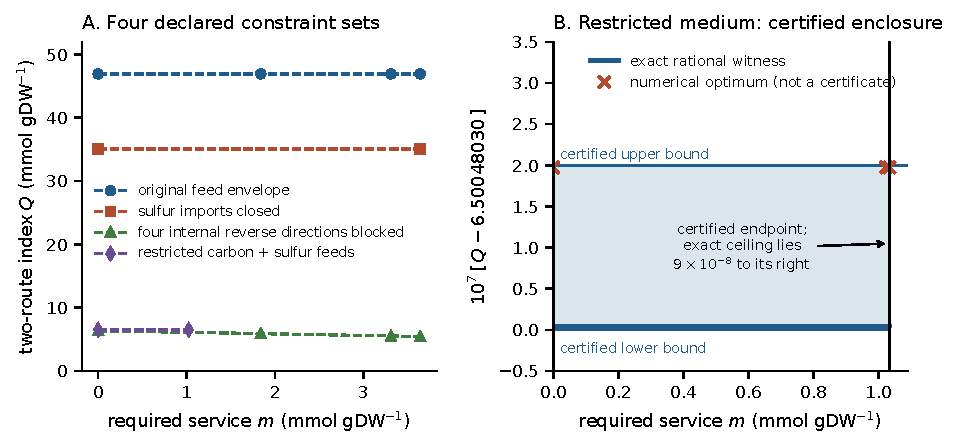
\includegraphics[width=\textwidth]{figures/fig1.pdf}
\caption{(A) Service--turnover comparisons at a one-hour horizon under the four
declared constraint sets of Table~\ref{tab:media}. Dashed segments join
computed values and are not additional certified points; the
internal-direction restriction is distinct from the external-supply
restrictions, and each medium has its own absolute service scale. (B) The
certified enclosure of Theorem~\ref{thm:plateau}, on an offset ordinate
$10^{7}[Q-6.50048030]$, so that the certified band is $[0,2]$. The shaded band
is drawn only over the certified service interval: the upper bound also holds
outside it, the lower bound is not claimed there. The lower horizontal line is
the exact rational witness value and the crosses are floating-point optima,
which are not certificates. The vertical line marks the certified endpoint; the
exact service ceiling lies $9\times10^{-8}$ further right and is not resolvable
at this scale. The band is an arithmetic enclosure for one model, not a
measured uncertainty interval.}
\label{fig:one}
\end{figure}

\begin{figure}[t]
\centering
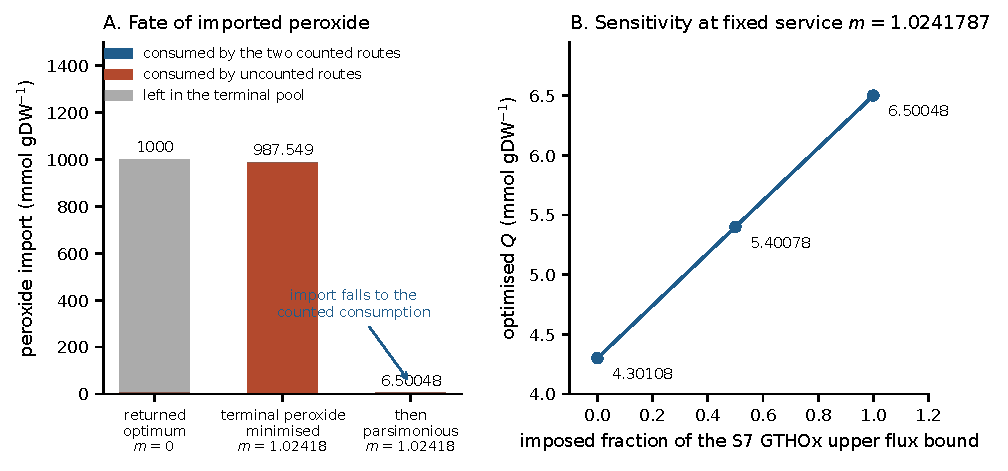
\includegraphics[width=\textwidth]{figures/fig2.pdf}
\caption{(A) Fate of imported peroxide in the three saved solutions of
Table~\ref{tab:peroxide}. Terminal-only minimisation substitutes uncounted
consumption for accumulation; the subsequent parsimony step removes it and
import falls to the counted consumption. The three bars are different primal
vectors at different service values. (B) Optimised turnover when only the
\texttt{GTHOx} upper flux bound is scaled, at fixed absolute service
$1.0241787$. The fractions are imposed model perturbations, not measured
activity changes, and the line joining three points is a visual guide.}
\label{fig:two}
\end{figure}

\section{Carrier inventory and finite-time recycling}\label{sec:carrier}

\subsection{A consequential rate assumption}
In the restricted-medium witness the two-route turnover decomposes as
approximately $49.9\%$ catalase, $33.8\%$ glutathione recycling supported by
the NADH-dependent \lean{GTHOx} column, and $16.3\%$ recycling supported
through the pentose-phosphate and thioredoxin route. These are properties of
one model witness, not measured pathway fractions or uniquely necessary
allocations. Their importance is that scaling a single capacity moves the
answer: at the same absolute service, reducing only the \lean{GTHOx} upper flux
bound to one half or to zero lowers the optimum from $6.500480$ to $5.400780$
and $4.301080$ (Figure~\ref{fig:two}B). Three samples do not establish a
globally affine sensitivity law, but they do identify a consequential
assumption rather than just another omitted reaction.

The assumption deserves care. The source files map the NADH-dependent
\lean{GTHOx} and the NADPH-dependent \lean{GTHOy} to the same glutathione
reductase homodimer, \lean{cplx_HOMODIMER_GSR}, and give both forward
directions the same estimated effective catalytic rate,
$2.19818\times10^{5}\,\mathrm h^{-1}$, with the source reaction forms
\[
\mathrm{GSSG}+\mathrm H^++\mathrm{NADH}\to2\,\mathrm{GSH}+\mathrm{NAD}^+,
\qquad
\mathrm{GSSG}+\mathrm H^++\mathrm{NADPH}\to2\,\mathrm{GSH}+\mathrm{NADP}^+ .
\]
The expanded allocation equations couple the use of that shared complex, so the
two individual flux maxima cannot simply be added, and the common estimated
effective rate is not a pair of fitted concentration-dependent kinetic laws.
Human erythrocyte glutathione reductase has been reported to use both NADPH and
NADH \citep{nakashima1976}, and its substrate-dependent behaviour has been
studied \citep{wong1989}; deleting the NADH-dependent activity merely because
NADPH is the more familiar donor would therefore not be justified. The
zero-capacity experiment is a sensitivity test. What is actually needed is
supported activity at the nucleotide and GSSG concentrations and the pH of a
chosen preparation.

\subsection{A sharp finite-time bound}
Carrier stock constrains turnover even when it is perfectly conserved, and the
constraint is invisible to a terminal balance. Consider a closed two-state
carrier with total amount $\Ctot$, reduced amount $g(t)$, oxidation turnover
$v(t)$ and regeneration $u(t)$, and positive first-order coefficients $a,b$:
\begin{equation}\label{eq:module}
g'=u-v,\qquad 0\le v\le a\,g,\qquad 0\le u\le b\,(\Ctot-g),\qquad
0\le g\le \Ctot .
\end{equation}
Take $g$ absolutely continuous and the rates integrable, so the inequalities
may hold almost everywhere, and write $V(T)=\int_0^Tv$. A simple closed
glutathione module uses $g=\mathrm{GSH}/2$ and
$\Ctot=\mathrm{GSH}/2+\mathrm{GSSG}$, which counts oxidised-disulfide
equivalents.

\begin{theorem}[Sharp transient recycling bound]\label{thm:carrier}
Under \eqref{eq:module}, for every $T\ge0$,
\begin{equation}\label{eq:sharp}
V(T)\ \le\ \frac{ab}{a+b}\,\Ctot\,T
+\frac{a}{a+b}\Bigl(g(0)-\frac{b\,\Ctot}{a+b}\Bigr)
\bigl(1-e^{-(a+b)T}\bigr),
\end{equation}
and equality holds for the saturated controls $v=ag$, $u=b(\Ctot-g)$.
\end{theorem}

Theorem~\ref{thm:carrier} is verified in Lean~4 as
\lean{PlateauEnclosure.carrier_transient_bound}, in the scope recorded in
Appendix~\ref{app:repro}; the sharpness statement and the corollaries below are
conventional.

\begin{proof}
Put $k=a+b$ and
\[
\lambda(t)=\frac ak\bigl(1-e^{-k(T-t)}\bigr),
\]
so that $\lambda(T)=0$, $0\le\lambda(t)\le a/k<1$ and
$\lambda'=k\lambda-a$. Then, almost everywhere on $[0,T]$,
\[
v+(\lambda g)'=(1-\lambda)v+\lambda u+\lambda'g
\le(1-\lambda)ag+\lambda b(\Ctot-g)+(k\lambda-a)g
=\lambda\,b\,\Ctot ,
\]
where the inequality uses $v\le ag$ with $1-\lambda\ge 0$, $u\le b(\Ctot-g)$
with $\lambda\ge0$, and then cancels the $g$ terms because
$(1-\lambda)a-\lambda b+k\lambda-a=0$. Integrating over $[0,T]$ and using
$\lambda(T)=0$ gives
\[
V(T)\le\lambda(0)g(0)+b\,\Ctot\int_0^T\lambda
=\frac ak\bigl(1-e^{-kT}\bigr)g(0)
+\frac{ab\,\Ctot}{k}\Bigl(T-\frac{1-e^{-kT}}{k}\Bigr),
\]
which is \eqref{eq:sharp} after collecting the two $(1-e^{-kT})$ terms. For
sharpness, the saturated controls give
$g'=b(\Ctot-g)-ag$, hence
$g(t)=\tfrac{b\Ctot}{k}+(g(0)-\tfrac{b\Ctot}{k})e^{-kt}$, which stays in
$[0,\Ctot]$ whenever $g(0)$ does, and $V(T)=a\int_0^Tg$ equals the right-hand
side of \eqref{eq:sharp}.
\end{proof}

\begin{corollary}\label{cor:carrier}
Under \eqref{eq:module}:
\begin{enumerate}[label=(\alph*)]
\item If $g(T)=g(0)$ and $T>0$ then $V(T)/T\le \Ctot/(1/a+1/b)$, and in general
the right-hand side of \eqref{eq:sharp} divided by $T$ exceeds that harmonic
ceiling by at most $O(1/T)$.
\item If $g(0)=0$ then $V(T)\le\tfrac12ab\,\Ctot T^2+O(T^3)$ as $T\to0$: the
upper envelope starts quadratically, because regeneration must precede
oxidation. An initially reduced pool instead has leading allowance $a\,g(0)T$.
\item If $\theta=g(0)/\Ctot$ is known then \eqref{eq:sharp} inverts to a
necessary lower bound on carrier amount,
\begin{equation}\label{eq:required}
\Ctot\ \ge\
\frac{V(T)}{\dfrac{ab}{a+b}T
+\dfrac{a}{a+b}\Bigl(\theta-\dfrac{b}{a+b}\Bigr)\bigl(1-e^{-(a+b)T}\bigr)} ,
\end{equation}
whenever the denominator is positive.
\item $\Ctot=0$ forces $g\equiv u\equiv v\equiv0$, so no positive turnover is
possible for any finite $a,b$.
\end{enumerate}
\end{corollary}

Part (a) is the version of the bound that appears when a terminal balance is
imposed; the point of \eqref{eq:sharp} is that no terminal condition is
needed, since a cell may legitimately draw down a reduced pool during a short
experiment. Part (d) is the sharpest contrast with the stoichiometric
relaxation: a balanced stoichiometric model can assign equal positive rates to
opposing carrier reactions while the carrier amount is zero at every sampled
time, and adding more balance time points alone does not remove that artefact.
Pool-dependent rate constraints are the missing condition, which is precisely
why the certified witness of Theorem~\ref{thm:plateau}, with zero modelled
initial carriers, is not evidence of kinetic feasibility.

\begin{table}[t]
\centering
\small
\begin{tabular}{@{}lr@{}}
\toprule
Initial reduced fraction $\theta$ & Maximum turnover per unit total carrier \\
\midrule
$0$ & $0.45551$ \\
$1/3$, the saturated stationary fraction & $2/3$ \\
$1$ & $1.08898$ \\
\bottomrule
\end{tabular}
\caption{Bound \eqref{eq:sharp} for an illustrative module with
$a=2\,\mathrm h^{-1}$, $b=1\,\mathrm h^{-1}$ and $T=1$~h, reported per unit
total carrier so that no physiological pool is invented. More than one turnover
per carrier is possible because the carrier recycles; equal total pools do not
give equal short-time turnover when the initial oxidation states differ. These
numbers illustrate the theorem and are not fitted red-cell predictions.}
\label{tab:carrier}
\end{table}

\begin{figure}[t]
\centering
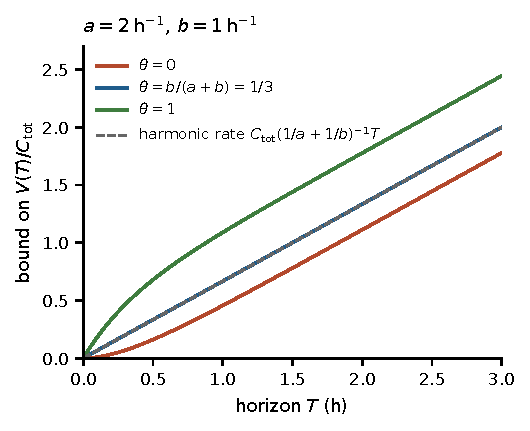
\includegraphics[width=0.52\textwidth]{figures/fig3.pdf}
\caption{The bound \eqref{eq:sharp} per unit total carrier for three initial
reduced fractions, with the harmonic average-rate ceiling for comparison. The
curves are upper envelopes for an abstract two-state module with the stated
coefficients, not measured red-cell trajectories.}
\label{fig:three}
\end{figure}

\subsection{What this costs the model witness}
For the returned \lean{GTHP} extent of approximately $3.2598729\ \mmolg$ over
one hour, a balanced closed-carrier explanation requires
$\Ctot/(1/a+1/b)\ge3.2598729\ \mathrm{mmol}\,\mathrm{gDW}^{-1}\mathrm h^{-1}$
by Corollary~\ref{cor:carrier}(a); if the pool is not restored, \eqref{eq:sharp}
or \eqref{eq:required} applies instead. This is a necessary diagnostic, not an
assertion that stored cells have zero carrier. It also suggests a concrete
measurement set: the total relevant carrier amount, its initial oxidation
state, and supported bounds on regeneration and oxidation at the relevant
substrate concentrations. Mixed disulfides, synthesis, export and additional
carrier states must either be included or justify the closed-module
approximation, and the measurements must constrain instantaneous rate bounds
rather than report a fitted average with no envelope interpretation. No
source-supported values of $a$, $b$ or $\Ctot$ are asserted here for any stored
preparation.

\section{A complementary recovery consistency test}\label{sec:recovery}

The capacity analysis identifies rate information that a stoichiometric
envelope does not provide. Recovery assays are a possible source of such
information, but their interpretation depends on how a treatment changes
oxidative input and effective reduction. We therefore examine a paired-signal
model and derive a necessary consistency test. This section specifies
observational requirements; it does not calibrate the S7 instance, and the two
analyses do not share a validated biological preparation.

\subsection{Identity}
Let $D$ be an untreated signal and $C_s$ a treated signal, with a common
positive initial value $D_0$, a single constant residual-input fraction
$0\le r<1$, and
\begin{equation}\label{eq:pairedode}
D'=q-kD,\qquad C_s'=rq-kC_s,\qquad D(0)=C_s(0)=D_0 ,
\end{equation}
where the oxidative input $q$ and the effective reduction $k$ may both vary
with time. Put $K(t)=\int_0^tk$ and
$z(t)=(C_s(t)-rD(t))/((1-r)D_0)$.

\begin{proposition}\label{prop:identity}
Under \eqref{eq:pairedode}, $z(t)=e^{-K(t)}$ for all $t$. If in addition
$k\ge0$ on $[0,t_2]$ then
\begin{equation}\label{eq:monotone}
0<z(t)\le1\quad\text{and}\quad z(t_2)\le z(t_1)\qquad(0\le t_1\le t_2).
\end{equation}
\end{proposition}

\begin{proof}
Set $Y=C_s-rD$. Subtracting the two equations cancels the oxidative input and
gives $Y'=-kY$, so $(e^KY)'=0$ and $e^{K}Y$ is constant. The common initial
value gives $Y(0)=(1-r)D_0$, whence the identity; the two consequences are
immediate from monotonicity of $K$ and positivity of the exponential.
\end{proof}

The identity conditionally identifies \emph{integrated effective reduction}. It
does not identify an intrinsic enzyme constant, and it makes no assumption of
constant oxidative input.

\subsection{Discrepancy, observation error and the test}
Suppose instead that the treated signal obeys
$C_s'=rq+\eta-(k+\delta)C_s$, and set $e=\eta-\delta C_s$. Variation of
constants gives
$z(t)-e^{-K(t)}=\frac{1}{(1-r)D_0}\int_0^te^{-(K(t)-K(s))}e(s)\,\dd s$,
and when $k\ge0$ the kernel lies in $(0,1]$, so
\begin{equation}\label{eq:gamma}
\bigl|z(t)-e^{-K(t)}\bigr|\ \le\ \Gamma(t)
:=\frac{\int_0^t|\eta(s)-\delta(s)C_s(s)|\,\dd s}{(1-r)D_0} .
\end{equation}
This allows both imperfect proportional suppression and a treatment effect on
effective reduction; a high treatment occupancy does not by itself bound either
term for every source of measured oxidation. If the transformed observation
error is at most $\varepsilon$, put $\zeta=\Gamma+\varepsilon$,
$L_z=\hat z-\zeta$ and $U_z=\min\{1,\hat z+\zeta\}$. Provided
$0<L_z\le U_z$,
\begin{equation}\label{eq:loginterval}
-\log U_z\ \le\ K(t)\ \le\ -\log L_z .
\end{equation}
An empty interval means the stated model and error assumptions are
incompatible. A nonpositive lower endpoint supplies no finite upper bound on
$K$, which is a failed identification margin and not evidence of an infinite
biological rate. The inference is sensitive near zero and as $r$ approaches
one, because the signal difference is divided by $1-r$.

Two practical points govern how the test is applied. First, preserve the raw
paired values and their common initial peak $P$: a normalised untreated signal
$D/P$ and a ratio $C_s/D$ share a denominator, their product being $C_s/P$, so
treating them as independent observations invents information and discards
correlated normalisation uncertainty. For fixed $r$ and raw absolute errors
bounded by $\epsilon_C,\epsilon_D,\epsilon_P$ with $\epsilon_P<P$, a
conservative transformed-error bound is
\begin{equation}\label{eq:errors}
\epsilon_z\ \le\ \frac{\epsilon_C+r\epsilon_D}{(1-r)(P-\epsilon_P)}
+\frac{Z_{\max}\epsilon_P}{P-\epsilon_P},
\end{equation}
provided the true transformed magnitude is at most $Z_{\max}$; this is a
deterministic bound, not a confidence interval. Second, use one common $r$ at
every time. For a fixed raw pair with $0\le C_s\le D$,
\[
\frac{\partial}{\partial r}\frac{C_s-rD}{(1-r)P}=\frac{C_s-D}{(1-r)^2P}\le0 ,
\]
so a specified interval for $r$ gives an exact endpoint range for that pair;
choosing a separate favourable value at each observation weakens the model
being tested.

The test itself is \eqref{eq:monotone}: a later transformed interval lying
strictly above an earlier one rejects the model at the stated error budget. For
a synthetic illustration take a common normalised initial peak of $1$,
observations $(D,C_s)=(0.8,0.5)$ followed by $(0.7,0.6)$, raw absolute errors
at most $0.01$, and one common $r\in[0,0.05]$. The smallest possible
later-minus-earlier numerator is $(C_{s,2}-C_{s,1})+r(D_1-D_2)\ge0.08+0.08r>0$,
while the denominator is positive and common, so every allowed realisation
violates \eqref{eq:monotone}. This is an illustrative incompatibility
certificate. It is not a finding about any published observation, and if
intervention discrepancy is permitted then its propagated interval must be
included before a rejection is claimed. Passing the test is only a necessary
consistency check: it does not validate the intervention mechanism, the
complete kinetics or any future prediction.

\subsection{Applicability}
The stored-cell peroxide recovery experiments that motivate this model used
washed stored human cells with micromolar peroxide at $37^{\circ}$C and
introduced carbon monoxide after a shared challenge period \citep{harper2015};
a later comparison used a different treatment timing and displayed
normalisation \citep{oh2022}. The two must not be merged by assuming a common
initial condition, and neither the original matched unnormalised donor signals
nor calibrated intervention errors were available to us. The consistency test
above is therefore a measurement consequence of the identity, not a reanalysis
claiming to resolve those experiments.

\section{Discussion}\label{sec:discussion}

\subsection{What the results mean}
The practical finding is not that ATP service and oxidative resilience are
unrelated. It is that the tested resource relaxation does not impose the
substantial tradeoff one might expect, that the tradeoff which does appear is
an artefact of imposed internal reverse restrictions and is not reproduced by
supply accounting, and that the assumptions which actually move the answer are
about rates, carrier pools and the fate of the oxidant. That narrows what
should be measured next.

The results are useful in different ways to different readers. A metabolic
modeller can check a proposed integrated output against an exact certificate
and inspect the routes that relax it, provided the same source constraints and
units are used. A bioinformatician can separate solver-discovered candidates
from checkable rational witnesses and upper bounds. An experimental
red-cell researcher gets a concrete list of quantities to distinguish: total
carrier amount, initial oxidation state and regeneration rate are three
different measurements, and matched raw recovery signals with their own initial
normalisation are worth more than an additional treatment-to-control ratio. A
bioengineer designing a challenge assay should specify absolute service,
external exposure and a damage-related endpoint before comparing preparations,
since relative service recalibration and total peroxide disappearance answer
different questions.

\subsection{The next bounded target}
The recommended next question is smaller than fitting a new red-cell model and
more informative than another unrestricted parameter grid:

\begin{quote}
For one documented stored-cell preparation, do measured carrier inventories and
supported nucleotide-dependent regeneration bounds exclude the high-turnover
restricted-medium witness, while preserving a feasible baseline service
condition?
\end{quote}

The glutathione and glutathione-reductase module is the place to start, because
the sensitivity experiment of Section~\ref{sec:carrier} shows that its
assumptions materially change $Q$. Five steps make the question decidable.
Choose one preparation and fix storage age, medium, temperature, normalisation,
treatment timing and assay compartment, rather than assembling a fictitious
donor from incompatible studies. Acquire the quantities that enter the bound:
GSH/GSSG and other relevant carrier pools, NADH and NADPH availability, shared
reductase activity at supported substrates, and the absolute service
requirement, retaining uncertainty as ranges with a stated basis. Insert the
smallest supported constraint, such as a justified pool-dependent rate envelope
or the integrated bound \eqref{eq:sharp}, rather than an arbitrary capacity
deletion. Retest the baseline before the challenge, since if service alone
becomes infeasible the diagnosis lies in the preparation or the capacity
assumptions and not in oxidative competition. And test a held-out time or
perturbation, because predicting a withheld recovery segment is more
informative than refitting the same two ratios. If the new bound does not move
the witness, its slack and the remaining active capacities identify the next
consequential assumption; if it excludes every baseline state, the units, pool
closure and kinetic envelope are the place to look. Both are informative
outcomes.

Adding exposure and a protective endpoint requires compatible data:
extracellular peroxide, transport, intracellular burden and a supported
functional or injury endpoint, with the matching conditions discussed after
\eqref{eq:burden}. A dynamic implementation can track substrate depletion
\citep{mahadevan2002} and a calibrated kinetic ensemble can express parameter
uncertainty \citep{bordbar2015}, but time discretisation alone, unconstrained
ensembles and flux minimisation do not supply the missing biological premise.
Balances alone cannot prevent turnover of a zero carrier pool.

\subsection{Scope statement}
The source-model inventory theorem is compiled at its stated conditional scope,
and the restricted-medium service--turnover enclosure is exactly rationally
certified over the whole certified service range. The numerical diagnostics and
the carrier and recovery arguments explain the limits of interpreting these
results physiologically. A source-supported theorem of stored-red-cell
oxidative tolerance with preserved ATP-dependent function remains open.

\appendix

\section{Reproducibility and verification scope}\label{app:repro}

\subsection*{Source data}
The primary data are the supplementary files S6 and S7 accompanying
\citet{haiman2025}. The S7 XML has SHA-256
\hashfour{b2703b5a730cf128}{90034f01df92506d}{e5facd9ecea5751a}{795e982b88557f64}. All
decimal coefficients are interpreted as exact rational numbers throughout; no
rounded float is ever a certificate input. A release should preserve the
original source identifiers, the row classification, the medium masks and the
exact XML version, since a list of reaction counts does not determine the
restriction.

\subsection*{Formal verification and its boundary}
The declaration
\lean{StoredRedCells.S7Certificate.source_joint_inventory_bound} in
\lean{proofs/StoredRedCells/S7Source.lean} states Theorem~\ref{thm:inventory}
as a concrete inequality between finite vector sums over the source family. The
recorded strict receipt reports successful compilation under Lean~4
\citep{moura2021} with the repository's pinned Mathlib \citep{mathlib2020},
warnings treated as errors, no \lean{sorry} and no additional axioms; the
proof-file SHA-256 is
\hashfour{9419514870b60a80}{3f4904eac1f31acf}{ad9383b84e4e2ff1}{1d10c48aead96bd1}. The
supporting modules separate concerns: \lean{FiniteCertificate.inventory_with_reverse_supplies}
is the general weighted-balance inequality with signed extents and reverse
charges, \lean{S7Bridge} converts between the integer representation and
physical scales, \lean{S7Application.inventory_from_chunks} applies the general
result to a family assembled from checked blocks, \lean{S7Data.Part0} through
\lean{Part19} hold the concrete data in modules of at most $1024$ columns each,
and \lean{S7Certificate.source_cost_exact} evaluates the complete residual-cost
sum. The recorded integer scales are $W=403619500$, $S=10^{16}$ and
$B=5\times10^{21}$: chemical weights divide by $W$, stoichiometry by $S$, rate
bounds by $B$ and objective and supply fields by $WS$. These are
representation choices, not physiological hypotheses.

What the kernel checks is the finite vector arithmetic and the implication.
What remains outside it is XML parsing, source-version selection, the
interpretation of reaction names as source coordinates, and biological
admissibility. The reaction names in \eqref{eq:main} identify source
coordinates through the external audit and manifest; a separate compiled
named-coordinate simplification is not claimed. The recovery identity, the
discrepancy bound and the logarithmic interval of Section~\ref{sec:recovery}
are compiled separately as
\lean{PairedRecovery.normalized_integrated_identity},
\lean{paired_robustness} and \lean{observation_rate_interval}, with global
derivative hypotheses on the real line; an interval-only minimisation of those
hypotheses is not claimed. Theorem~\ref{thm:plateau} is established by exact rational arithmetic in
Python, and is \emph{not} claimed as a Lean-replayed source certificate.

The abstract results of Sections~\ref{sec:plateau} and~\ref{sec:carrier} are
compiled separately in \lean{proofs/StoredRedCells/PlateauEnclosure.lean} as
\lean{feasible_nonempty}, \lean{uniform_enclosure}, \lean{value_antitone},
\lean{value_concave}, \lean{infeasible_above_ceiling} and
\lean{carrier_transient_bound}, in one strict compilation under Lean~4.30.0
with warnings treated as errors, no \lean{sorry}, and the standard axioms
\lean{Classical.choice}, \lean{Quot.sound} and \lean{propext} only; the
proof-file SHA-256 is
\hashfour{c01bafb0d3e3200a}{ba595782a95ca691}{ee7766c2e749aaf1}{44175db084909a21}. Three
scope points should be recorded exactly. The compiled carrier statement assumes
that $g$ is differentiable everywhere with $g'=u-v$ and that $u,v$ are
continuous, which is stronger than the almost-everywhere hypotheses used in
Theorem~\ref{thm:carrier}; the conventional proof above is the one that covers
the weaker scope. Conversely the compiled statement is more general in one
respect: it never uses $0\le g\le\Ctot$, since only the two caps enter the
pointwise estimate. Finally, the nonnegativity hypotheses $0\le v$ and $0\le u$
are inert for the upper bound, as is $0\le m_h$ in the enclosure lemma; they
are retained in the compiled statements as part of the declared model scope,
and the compiled files say so. The sharpness claim in
Theorem~\ref{thm:carrier}, the corollaries and everything in
Sections~\ref{sec:recycling}--\ref{sec:burden} are ordinary proofs or numerical
records, not compiled statements.

\subsection*{Exact values for the plateau certificate}
The rational witness, the turnover weights and the service weights are
deposited in the audit record together with every nonzero entry. The decisive
exact values are
\[
M(\xi_h)=\frac{4421041890341877}{4273504273504270},
\qquad
Q(\xi_h)=\frac{9400187505686245981195327946603}
{1446075838260537275756274164820},
\]
\[
U=\frac{81256006217701144379925098514861}
{12500000000000000000000000000000},
\qquad
U_M=\frac{2586309736197958070773983682319}
{2500000000000000000000000000000},
\]
with decimal summaries $1.03452380234$, $6.500480304680002$,
$6.500480497416092$ and $1.0345238944791832$, and $U-L<1.93\times10^{-7}$ for
the displayed rounded $L=6.50048030$. The audit reports exact primal
feasibility with no inconsistent reconstructed equation, no bound violation and
no chemical or auxiliary balance violation, from $2009$ selected free variables
and $1651$ pivots; those labels describe reconstruction stages and are not a
claimed nullity. The witness has $1580$ nonzero entries, the turnover
certificate has $194$ chemical and $128$ auxiliary weights with $8$ nonzero
interval-cost terms, and the service certificate has $200$ chemical and $251$
auxiliary weights with $2$ nonzero terms. An earlier, narrower audit of the
same medium certified the same band only for $m\le1.02417$; the present
certificate supersedes it and both records are retained.

A verification-only entry point should consume the frozen model, the explicit
row classification and the medium mask, align rows and columns by recorded
source identifiers while rejecting duplicates or omissions, interpret every
decimal and every certificate fraction exactly, fill omitted sparse entries
with exact zero, check every bound, floor and equality, recompute $M$ and $Q$
from their named coordinates, check that the dual chemical weights are
nonnegative, recompute every dual residual and interval maximum while retaining
all nonzero terms, and emit a PASS or FAIL record tied to the input hashes.
Checking that array lengths agree is not a proof of semantic alignment;
identifier-based verification and a frozen restriction manifest are what
address that risk.

\subsection*{Numerical computations}
All floating-point linear programs use single-threaded HiGHS
\citep{huangfu2018} through SciPy \citep{virtanen2020} on the complete sparse
model. The cleanup fixes service and turnover within $10^{-8}$, minimises
terminal peroxide, then minimises total absolute flux while preserving that
result. The plateau witness search maximises service subject to a turnover
floor, and the sensitivity experiment changes only the \lean{GTHOx} upper flux
bound. No parameter grid, donor-cohort fit, concentration conversion or
measured kinetic validation is implied anywhere. The figures are generated
directly from the saved records, and the symbolic identities behind
Theorem~\ref{thm:carrier} and Corollary~\ref{cor:carrier} are checked with a
computer algebra system.

\bibliographystyle{unsrtnat}
\bibliography{refs}

\end{document}
